%!TEX root = ../thesis.tex
%*******************************************************************************
%*********************************** First Chapter *****************************
%*******************************************************************************

\chapter{Introduction}  %Title of the First Chapter

\ifpdf
    \graphicspath{{Introduction/Figs/Raster/}{Introduction/Figs/PDF/}{Introduction/Figs/}}
\else
    \graphicspath{{Introduction/Figs/Vector/}{Introduction/Figs/}}
\fi
%********Literature Review************
%********Review HGSOC, microenvironments, spatial analysis, collagen, hypoxia, immune system and functionality/interactions************


%********************************** %First Section  **************************************
\section{What is Ovarian cancer?} %Section - 1.1 

Introduction to the thesis which is about Ovarian Cancer, the tumour microenvironment and collagen (see 
Section~\ref{section1.3}). Ovarian cancer is believed to originate in the fallopian tube \citep{AAB95,Con90,LM65}.



%********************************** % Third Section  *************************************
\section{What is understood about the microenvironment?}  %Section - 1.3 
\label{section1.3}
The microenvironment of a tumour comprises the cells surrounding and infiltrating the tumour as well as the physical and chemical properties of the region, immune cells, the extracellular matrix and hypoxia are all examples of microenvironmental features.

The microenvironment has been a topic of great interest recently, with rapidly expanding studies of its importance and potential to facilitate metastasis or drive tumour progression. \citep{RN22, RN10, RN37,RN11, RN2, RN26}

\section{Gene expression subtypes}

\section{Tumour proliferation and structure}
\begin{figure}
    \centering
    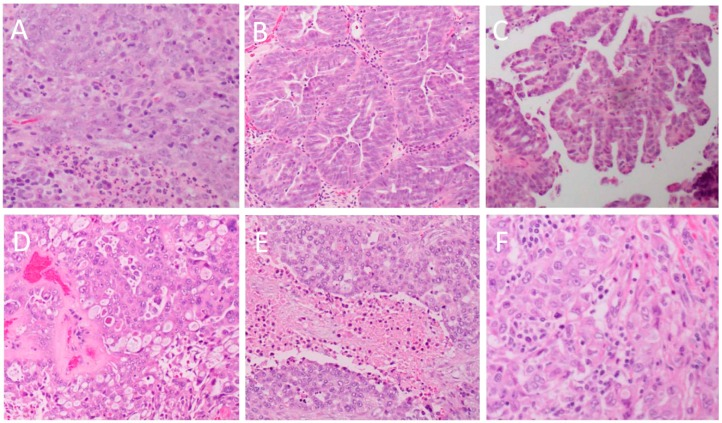
\includegraphics[width=\textwidth]{Introduction/Figs/Raster/ijms-20-00952-g001.jpg}
    \caption[Morphology types in HGSOC]{Heterogeneous morphology of HGSOC tissues, examples from Murakami \textit{et. al.}\citep{murakami2016establishment}. A) Solid growth architecture B) C) D) E). }
    \label{fig:morphology_murakami}
\end{figure}
\citep{murakami2016establishment, Lisio2019Feb}


%********************************** %Second Section  *************************************
\section{What drives HGSOC?} %Section - 1.2

TP53 mutations are believed to be ubiquitous in high grade serous. The HGSOC genome is extremely complex and highly rearranged. In the face of such complexity it is difficult to elucidate exactly what is causing what.  \citep{RN17}


\nomenclature[z-HGSOC]{HGSOC}{High Grade Serous Ovarian Cancer}
\nomenclature[z-TMA]{TMA}{Tissue Micro Array}
\nomenclature[z-IMC]{IMC}{Immuno Metal Conjugation}
\nomenclature[z-IHC]{IHC}{Immuno histo chemistry}
\nomenclature[z-IF]{IF}{Immunofluorescence}
\nomenclature[z-SHG]{SHG}{Second Harmonic Generation}
\nomenclature[z-GLCM]{GLCM}{Grey Level Co-occurence Matrix}

